\section{Task 1}
\FloatBarrier % Now figures cannot float above section title


\subsection{How original and unique is the designed robot?}

After discussion and doing some references, our group decide to make our robot arm as a four-arm robot and define the robot arms and joints, because there are some advantages of four-arm robot:

\begin{itemize}
\item better accuracy and stability of the movement;
\item bigger working arrangement;
\item better loading allowance;
\item better collaboration.
\end{itemize}


\textbf{And there are also some unique assessments of our four-robot arms can meet:}

\begin{itemize}
\item The welding robot arm allows more precise control of the welding position and angle.
\item The stability in high temperature, low temperature and hazardous gas environments ensure safe and stable welding.
\item Compared to manual welding, welding robots can automate welding work, thus increasing productivity and reducing labor costs.
\item To make sure the arms and joints will not clash into each other.
\item Risk of joint interference: Do kinematic analysis to determine the minimum spacing and range of the movements between the joints and the robot arms, so that we can avoid the interference of the clash of the joints.
\item Simulation analysis: After setting the exact parameters of the arms and joints, we use MATLAB to do simulation of real situations, and make sure the clash of the joints and arms won't happen.
\item Design concept: After doing some researches of designing the robots, we consider the working arrangement, the stability of the robots and its operability. In order to achieve the function of welding in an exact area, we finally make the definitions of the parameters of all the arms and joints.
\end{itemize}


\subsection{Property of all the arms and the joints}

We have designed 4 joints for the robot, 2 of which are revolute type and 2 are prismatic type. At the same time, there are four corresponding robotic arms, whose parameters are shown in the following table:

\begin{minipage}[htbp]{\textwidth}
    \makeatletter\def\@captype{table}
    \centering
    \scalebox{1}{
    \begin{tabular}{cccc}
    \hline
    Name & Body Mass (kg) & Center of mass & Inertia ($I_{xx}$ $I_{yy}$ $I_{zz}$) ($kg \cdot m^2$)                  \\ \hline
    R1   & 10        & (0 0 0)        & (0.27 0.27 0.8 )     \\
    R2   & 10        & (0 0 0)        & (0.27 0.27 0.8 )     \\
    P1   & 1.5       & (0 0 0)        & (0.07 0.07 0.07 )    \\
    P2   & 1.5       & (0 0 0)        & (0.07 0.07 0.07 )    \\
    Tool & 1.2       & (0 0 0)        & (0.002 0.002 0.004 ) \\ \hline
    \end{tabular}} 


    \caption{Experiment parameters}
    \label{t1} 
\end{minipage}


\begin{minipage}[htbp]{\textwidth}
    \makeatletter\def\@captype{table}
    \centering
    \scalebox{1}{
    \begin{tabular}{cccc}
    \hline
    Joint & Type & Position Limit (rad \& m) & Joint Axis                   \\ \hline
    1   & revolute       & $[-5\frac{\pi}{180}, 5\frac{\pi}{180}]$ & [0 0 1]     \\
    2   & revolute       & $[-30\frac{\pi}{180}, 30\frac{\pi}{180}]$        & [0 1 0]     \\
    3   & prismatic      & $[-0.5,0.5]$        & [1 0 0]    \\
    4   & prismatic      & $[-1, 1]$        & [0 1 0]    \\ 
    Fixed &revolute & N/A & N/A \\\hline
    \end{tabular}} 

    (Unit: mm)
    \caption{Experiment parameters}
    \label{t1} 
\end{minipage}

This is a schematic diagram of the robot in MATLAB.

\begin{figure}[htbp]
    \centering
    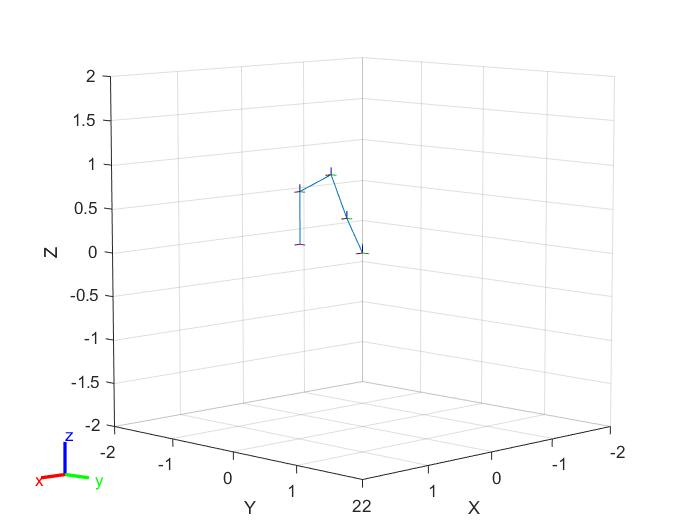
\includegraphics[width=10cm]{./fig/1.jpg}
    \caption{Force vs deformation and total moment diagram}
    \label{f4}
\end{figure}

\subsection{Collision discussion}

Our designed robot is free from collisions. In most cases, collisions occur on the two arms of the rotating joints whose rotation angle is greater than ±90 degrees. For our designed robot, the total range of motion for the two movable joints is ±35 degrees, so there is no collision. Additionally, the animation of the robot's movement trajectory can be viewed in the dynamic image in Figure 8.
